\documentclass[10pt]{article}
\usepackage[a4paper,margin=15mm]{geometry}
\usepackage{amsmath,amssymb,mathtools}
\usepackage{xcolor}
\usepackage{tikz}
\usetikzlibrary{arrows.meta,positioning,calc,fit,matrix,shapes.geometric}
\usepackage[T1]{fontenc}
\usepackage{lmodern}
\pagestyle{empty}

\definecolor{endo}{HTML}{355C7D}
\definecolor{frob}{HTML}{2A9D8F}
\definecolor{trace}{HTML}{E9C46A}
\definecolor{eqn}{HTML}{E76F51}
\definecolor{ink}{HTML}{263238}
\tikzset{
  block/.style={draw,rounded corners=2pt,very thick,align=center,minimum height=10mm,
    text width=36mm,fill=white},
  arr/.style={-{Stealth[length=2.5mm]},very thick,draw=ink},
  note/.style={draw,rounded corners,align=left,inner sep=5pt,fill=gray!5},
  atom/.style={circle,draw,very thick,minimum size=9mm,fill=white}
}

\newcommand{\F}{\mathbb F_{2^n}}
\newcommand{\Fr}{\operatorname{Fr}}
\newcommand{\Tr}{\operatorname{Tr}}
\newcommand{\lean}[1]{\texttt{#1}}

\begin{document}

\begin{center}
  {\LARGE\bfseries Dobbertin Theorem 1: Standalone LEGO Path}\\[2mm]
  {\large From an additive endomorphism to equation (1) $\Rightarrow$ equation (2)}
\end{center}

\vspace{3mm}
\begin{center}
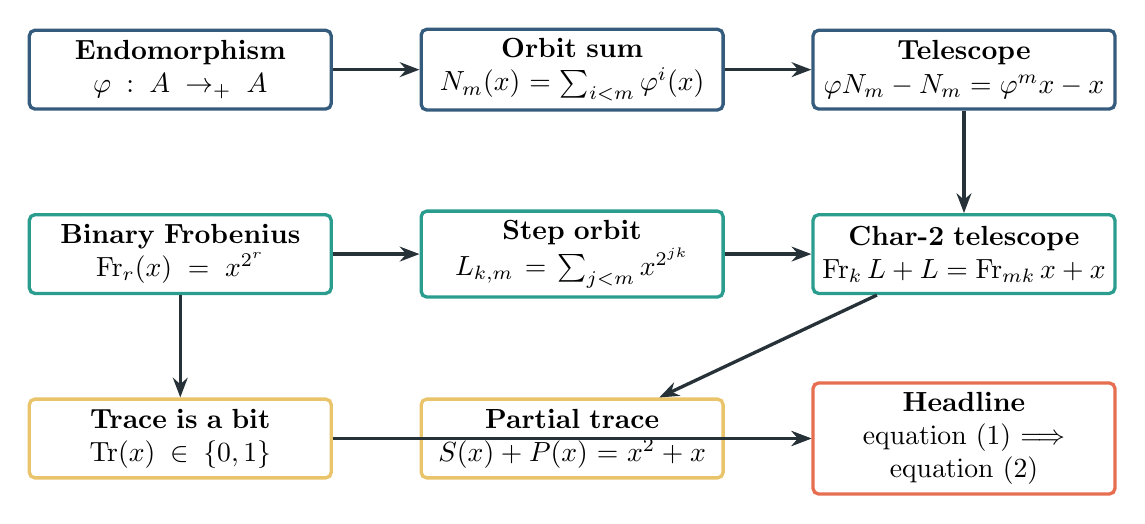
\begin{tikzpicture}[node distance=13mm and 11mm]
  \node[block,draw=endo] (end) {\textbf{Endomorphism}\\$\varphi:A\to_+ A$};
  \node[block,draw=endo,right=of end] (orbit) {\textbf{Orbit sum}\\$N_m(x)=\sum_{i<m}\varphi^i(x)$};
  \node[block,draw=endo,right=of orbit] (tel) {\textbf{Telescope}\\$\varphi N_m-N_m=\varphi^m x-x$};
  \draw[arr] (end)--(orbit); \draw[arr] (orbit)--(tel);

  \node[block,draw=frob,below=of end] (fr) {\textbf{Binary Frobenius}\\$\Fr_r(x)=x^{2^r}$};
  \node[block,draw=frob,right=of fr] (loop) {\textbf{Step orbit}\\$L_{k,m}=\sum_{j<m}x^{2^{jk}}$};
  \node[block,draw=frob,right=of loop] (ftel) {\textbf{Char-2 telescope}\\$\Fr_kL+L=\Fr_{mk}x+x$};
  \draw[arr] (fr)--(loop); \draw[arr] (loop)--(ftel);
  \draw[arr] (tel)--(ftel);

  \node[block,draw=trace,below=of fr] (tr) {\textbf{Trace is a bit}\\$\Tr(x)\in\{0,1\}$};
  \node[block,draw=trace,right=of tr] (pt) {\textbf{Partial trace}\\$S(x)+P(x)=x^2+x$};
  \node[block,draw=eqn,right=of pt] (head) {\textbf{Headline}\\equation (1) $\Longrightarrow$ equation (2)};
  \draw[arr] (fr)--(tr); \draw[arr] (ftel)--(pt); \draw[arr] (tr)--(head); \draw[arr] (pt)--(head);
\end{tikzpicture}
\end{center}

\vfill
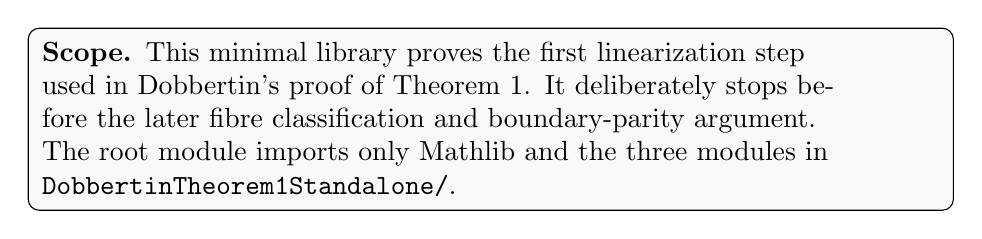
\begin{tikzpicture}
\node[note,text width=.94\textwidth] {
\textbf{Scope.} This minimal library proves the first linearization step used in
Dobbertin's proof of Theorem~1.  It deliberately stops before the later fibre
classification and boundary-parity argument.  The root module imports only
Mathlib and the three modules in \lean{DobbertinTheorem1Standalone/}.
};
\end{tikzpicture}

\newpage
\section*{1. The universal block: an orbit telescope}

Let $A$ be an additive commutative group and let $\varphi\in\operatorname{End}(A)$.
The only abstract construction is
\[
  N_m(x)=x+\varphi(x)+\cdots+\varphi^{m-1}(x).
\]
Applying $\varphi$ shifts every term one place.  Subtraction cancels the interior:
\[
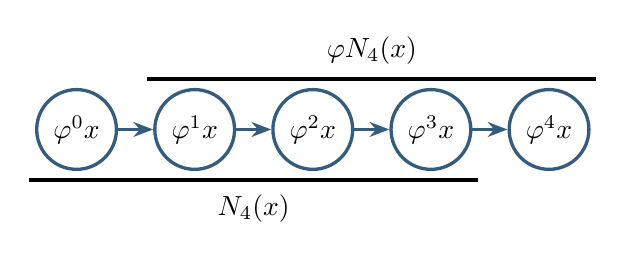
\begin{tikzpicture}[baseline=(current bounding box.center),x=15mm,y=8mm]
  \foreach \i in {0,...,4} {
    \node[atom,draw=endo] (a\i) at (\i,0) {$\varphi^{\i}x$};
  }
  \foreach \i in {0,...,3} {\draw[arr,draw=endo] (a\i)--(a\the\numexpr\i+1\relax);}
  \draw[very thick] (-.4,-.8)--(3.4,-.8);
  \node at (1.5,-1.25) {$N_4(x)$};
  \draw[very thick] (.6,.8)--(4.4,.8);
  \node at (2.5,1.25) {$\varphi N_4(x)$};
\end{tikzpicture}
\qquad
  \varphi N_m(x)-N_m(x)=\varphi^m(x)-x.
\]

\begin{center}
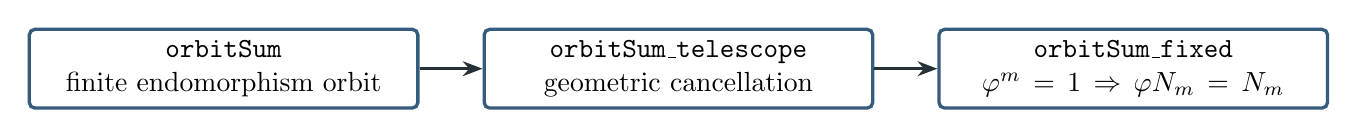
\begin{tikzpicture}[node distance=8mm]
 \node[block,draw=endo,text width=47mm] (d) {\lean{orbitSum}\\finite endomorphism orbit};
 \node[block,draw=endo,text width=47mm,right=of d] (t) {\lean{orbitSum\_telescope}\\geometric cancellation};
 \node[block,draw=endo,text width=47mm,right=of t] (f) {\lean{orbitSum\_fixed}\\$\varphi^m=1\Rightarrow\varphi N_m=N_m$};
 \draw[arr] (d)--(t); \draw[arr] (t)--(f);
\end{tikzpicture}
\end{center}

The first arrow uses only the additive-group laws.  The second is a one-line
consequence when the orbit closes.  No field, characteristic, or finiteness is
present yet.

\vspace{5mm}
\section*{2. Specialization to binary Frobenius}

Over $F=\F$, set $\Fr_r(x)=x^{2^r}$.  Characteristic two supplies additivity,
while finite-field Fermat supplies the closed orbit:
\[
 \Fr_r(x+y)=\Fr_r(x)+\Fr_r(y),\qquad
 \Fr_a(\Fr_b(x))=\Fr_{a+b}(x),\qquad \Fr_n(x)=x.
\]
Thus $\Fr_k$ is an additive endomorphism and the abstract norm becomes
\[
 L_{k,m}(x)=\sum_{j=0}^{m-1}\Fr_{jk}(x)
           =\sum_{j=0}^{m-1}x^{2^{jk}}.
\]
In characteristic two, minus equals plus, so the universal telescope reads
\[
 \boxed{\ \Fr_k(L_{k,m}(x))+L_{k,m}(x)=\Fr_{mk}(x)+x\ }.
\]

\newpage
\section*{3. The paper objects are settings of one loop}

\begin{center}
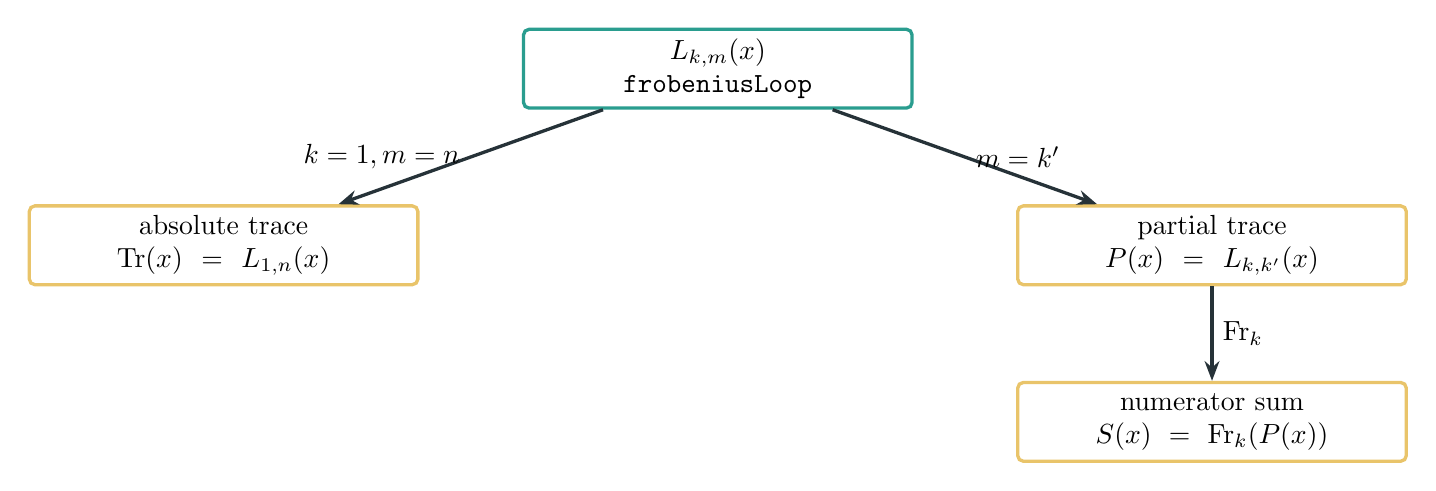
\begin{tikzpicture}[node distance=12mm and 13mm]
 \node[block,draw=frob,text width=47mm] (loop) {$L_{k,m}(x)$\\\lean{frobeniusLoop}};
 \node[block,draw=trace,text width=47mm,below left=of loop] (tr) {absolute trace\\$\Tr(x)=L_{1,n}(x)$};
 \node[block,draw=trace,text width=47mm,below right=of loop] (p) {partial trace\\$P(x)=L_{k,k'}(x)$};
 \node[block,draw=trace,text width=47mm,below=of p] (s) {numerator sum\\$S(x)=\Fr_k(P(x))$};
 \draw[arr] (loop)--node[left] {$k=1,m=n$} (tr);
 \draw[arr] (loop)--node[right] {$m=k'$} (p);
 \draw[arr] (p)--node[right] {$\Fr_k$} (s);
\end{tikzpicture}
\end{center}

The full orbit is fixed by Frobenius.  Therefore $\Tr(x)^2=\Tr(x)$, and field
factorization gives
\[
 \Tr(x)(\Tr(x)-1)=0
 \quad\Longrightarrow\quad
 \boxed{\Tr(x)=0\ \text{or}\ \Tr(x)=1}.
\]

Assume $kk'\equiv1\pmod n$.  Frobenius periodicity changes the far endpoint of
the step-orbit telescope into $\Fr_1(x)=x^2$:
\[
\begin{aligned}
 S(x)+P(x)
   &=\Fr_k(L_{k,k'}(x))+L_{k,k'}(x)\\
   &=\Fr_{k'k}(x)+x\\
   &=x^2+x.
\end{aligned}
\]

\begin{center}
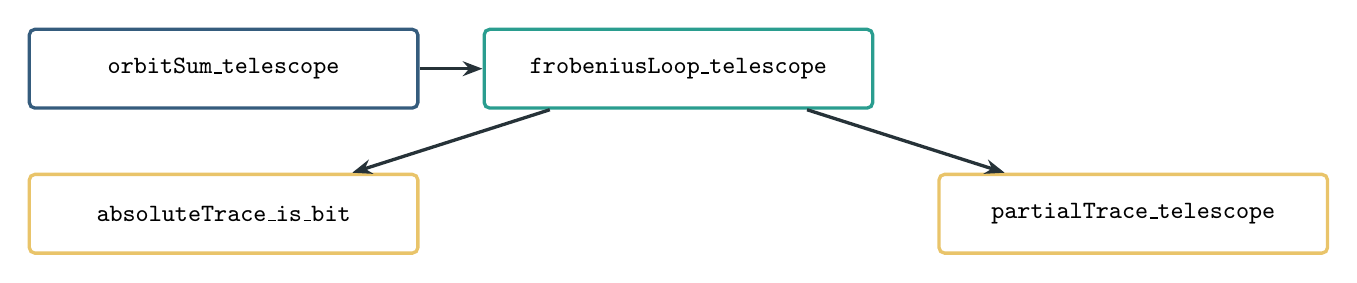
\begin{tikzpicture}[node distance=8mm and 8mm]
 \node[block,draw=endo,text width=47mm] (ot) {\small\lean{orbitSum\_telescope}};
 \node[block,draw=frob,text width=47mm,right=of ot] (flt) {\small\lean{frobeniusLoop\_telescope}};
 \node[block,draw=trace,text width=47mm,below left=of flt] (bit) {\small\lean{absoluteTrace\_is\_bit}};
 \node[block,draw=trace,text width=47mm,below right=of flt] (pt) {\small\lean{partialTrace\_telescope}};
 \draw[arr] (ot)--(flt); \draw[arr] (flt)--(bit); \draw[arr] (flt)--(pt);
\end{tikzpicture}
\end{center}

\newpage
\section*{4. Equation (1) to equation (2)}

For $\alpha\in\{0,1\}$, the cleared fibre equation is represented as
\[
 \tag{1}
 c\,x^{2^k+1}=S(x)+\alpha\Tr(x).
\]
Put $\varepsilon=\alpha\Tr(x)$.  The trace result says
$\varepsilon\in\{0,1\}$, hence $\varepsilon^{2^k}=\varepsilon$.  Combine
(1) with $S+P=x^2+x$ and $S=P^{2^k}$:

\begin{center}
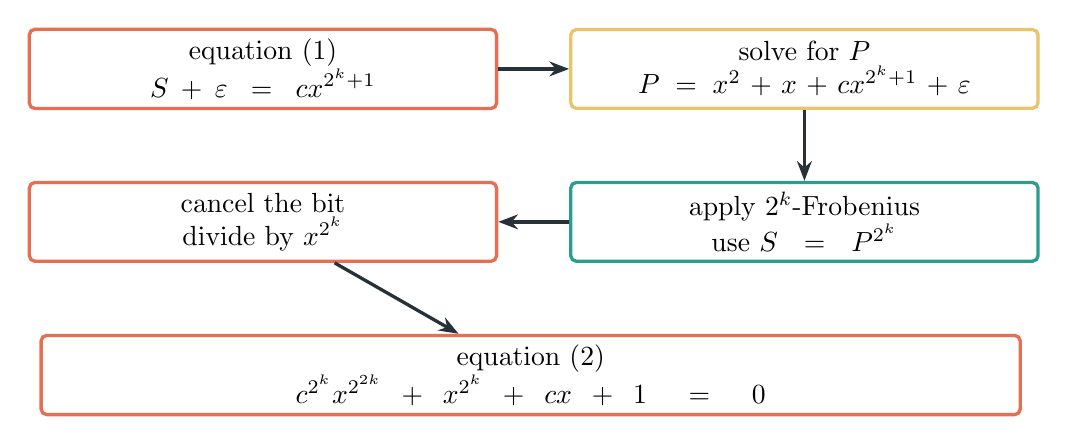
\begin{tikzpicture}[node distance=9mm]
 \node[block,draw=eqn,text width=57mm] (one) {equation (1)\\$S+\varepsilon=cx^{2^k+1}$};
 \node[block,draw=trace,text width=57mm,right=of one] (solve) {solve for $P$\\$P=x^2+x+cx^{2^k+1}+\varepsilon$};
 \node[block,draw=frob,text width=57mm,below=of solve] (raise) {apply $2^k$-Frobenius\\use $S=P^{2^k}$};
 \node[block,draw=eqn,text width=57mm,left=of raise] (cancel) {cancel the bit\\divide by $x^{2^k}$};
 \node[block,draw=eqn,text width=122mm,below=of cancel,xshift=34mm] (two) {equation (2)\\$c^{2^k}x^{2^{2k}}+x^{2^k}+cx+1=0$};
 \draw[arr] (one)--(solve); \draw[arr] (solve)--(raise); \draw[arr] (raise)--(cancel); \draw[arr] (cancel)--(two);
\end{tikzpicture}
\end{center}

The division is the sole reason for the hypothesis $x\ne0$.  The final theorem is:
\[
\boxed{
\begin{gathered}
 |F|=2^n,\quad kk'\bmod n=1,\quad \alpha\in\{0,1\},\quad x\ne0,\\
 \operatorname{EquationOne}(n,k,k',\alpha,c,x)
 \ \Longrightarrow\
 \operatorname{EquationTwoExpression}(k,c,x)=0.
\end{gathered}}
\]

\begin{center}
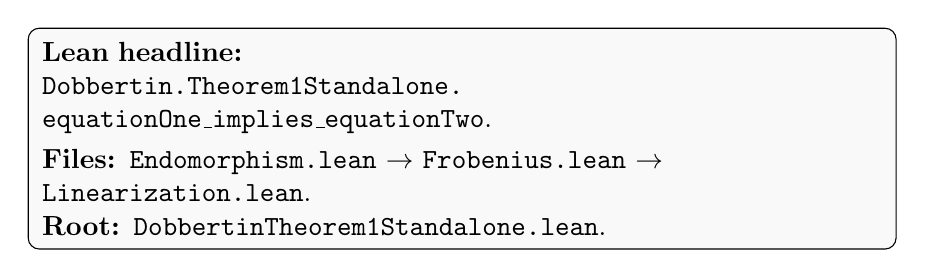
\begin{tikzpicture}
 \node[note,text width=.88\textwidth] {
 \textbf{Lean headline:}\\
 \lean{Dobbertin.Theorem1Standalone.}\\
 \lean{equationOne\_implies\_equationTwo}.\\[1mm]
 \textbf{Files:} \lean{Endomorphism.lean} $\to$ \lean{Frobenius.lean} $\to$
 \lean{Linearization.lean}.\\
 \textbf{Root:} \lean{DobbertinTheorem1Standalone.lean}.
 };
\end{tikzpicture}
\end{center}

\vfill
\begin{center}\small
The formal development is standalone relative to Mathlib and contains no admitted lemmas.
\end{center}

\end{document}
